% TU/e Style Master Thesis template for LaTeX.

\documentclass[a4paper,10pt,twoside]{report}

% Packages are defined at the thesis.sty file.
\usepackage{thesis}

% Define key:value pairs.
\newcommand{\shortdoctitle}{Block MLDU report}
\newcommand{\doctitle}{Block MLDU}
\newcommand{\docsubtitle}{Accelerate Block MLDU}
\newcommand{\me}{Lucas Bekker}
\newcommand{\keywords}{MLDU}
\newcommand{\version}{v1.0}
\newcommand{\studentid}{0657761}
\newcommand{\monthYear}{December 2018}
\newcommand{\firstCommitteeMember}{dr. J.M.L. Joseph Maubach}
\newcommand{\secondCommitteeMember}{}
\newcommand{\thirdCommitteeMember}{}

\author{\me}

% PDF settings.
\hypersetup
{
    pdfauthor={\me},
    pdftitle={\shortdoctitle},
    pdfsubject={\doctitle},
    pdfkeywords={\keywords}
}

\begin{document}

% Titlepage
\pagenumbering{gobble}
\include{titlepage}
\cleardoublepage
\pagenumbering{roman}
\normalsize

% Abstract
%\chapter*{Abstract}\label{chapter:abstract}

% TOC, list of figures and list of tables.
\cleardoublepage
\tableofcontents
\newpage

\chapter*{List of Acronyms}


\begin{acronym}[MLDU] % Give the longest label here so that the list is nicely aligned


\acro{TU/e}{Technische Universiteit Eindhoven}
\acro{LU}{contraction of the "Lower" and "Upper" matrices}
\acro{LDU}{contraction of the "Lower", "Diagonal" and "Upper" matrices}
\acro{MLDU}{contraction of the "Matrix", "Lower", "Diagonal" and "Upper" matrices}
\acro{COO}{coordinate list}
\acro{CCS}{compressed column storage}
\acro{VRAM}{video random access memory}
\acro{RAM}{random access memory}


\end{acronym}

% Page settings
\setcounter{page}{0}
\pagenumbering{arabic}

% Chapters
\cleardoublepage
\chapter{Introduction}

The goal of this Capita Selecta is to investigate the possibilities for a fast MATLAB based implementation of the Block MLDU algorithm.\\

\noindent High performance solvers are usually written in languages like C/C++ because they are compiled, avoiding the sometimes costly step of the interpreter. Languages like MATLAB are dynamically typed and interpreter based, which make them great for prototyping purposes.\\

\noindent The Block MLDU algorithm shows great possibilities, but the lack of a high performance implementation makes it prohibitive to use for large matrices. This is a problem because research projects sometimes encounter very large matrices that need to be solved with the Block MLDU algorithm.\\

\noindent This project tries to alleviate the problem by investigating the performance bottlenecks of a MATLAB based implementation and provide workarounds for them. This should result in a much faster implementation without requiring the extra work associated with a full C/C++ version.\\

\noindent The biggest advantage of this workflow is that the time required to implement a workaround for a bottleneck will be much lower in MATLAB than in C/C++, making it easier to try different approaches to the problems. The lessons learned at this stage will still be useful when the code does finally get ported to C/C++.\\

\noindent The biggest disadvantage to sticking to MATLAB is that the interpreter will always provide some overhead compared to C/C++. The hope is that this overhead will be small compared to the other bottlenecks encountered.

\newpage

\section{The Block MLDU algorithm}

The Block MLDU algorithm is very comparable to the well known LU decomposition. The main difference between the Block MLDU algorithm and LU decomposition is the "block" nature of the splitting.

\subsection{Example}

A simple example will be provided to highlight the differences between LU and Block MLDU. Let matrix $A$ be $4 \times 4$:\\

$
\hspace{20mm} A = 
\left\lbrack\begin{array}{rrrr}
           1&           0&           1&           0\\
           2&           1&          -1&           0\\
           0&          -1&           0&           1\\
          -2&           0&           1&           3
\end{array}\right\rbrack
$
$
\hspace{30mm} s =
\left\lbrack\begin{array}{rrr}
           2&           1&           1
\end{array}\right\rbrack
$\\

\noindent As stated by row $s$, matrix $A$ will first be split using a $2 \times 2$ block, followed by two $1 \times 1$ blocks.\\

\noindent \textbf{Step one:}\\

$
\left\lbrack\begin{array}{rr|rr}
          D1&          D1&          U1&          U1\\
          D1&          D1&          U1&          U1\\ \hline
          L1&          L1&          M1&          M1\\
          L1&          L1&          M1&          M1
\end{array}\right\rbrack
$
$
\hspace{10mm} L1 = 
\left\lbrack\begin{array}{rr}
           0&          -1\\
          -2&           0
\end{array}\right\rbrack
$
$
\hspace{6mm} D1 = 
\left\lbrack\begin{array}{rr}
           1&           0\\
           2&           1
\end{array}\right\rbrack
$
$
\hspace{6mm} U1 = 
\left\lbrack\begin{array}{rr}
           1&           0\\
          -1&           0
\end{array}\right\rbrack
$\\

$
Schur1 = L1 D1^{-1} U1 =
$
$
\left\lbrack\begin{array}{rr}
           3&           0\\
          -2&           0
\end{array}\right\rbrack
$
$
\hspace{20mm} A - Schur1 = 
\left\lbrack\begin{array}{rrrr}
           1&           0&           1&           0\\
           2&           1&          -1&           0\\
           0&          -1&  \textbf{-3}&  \textbf{1}\\
          -2&           0&   \textbf{3}&  \textbf{3}
\end{array}\right\rbrack
$\\

\noindent \textbf{Step two:}\\

$
\left\lbrack\begin{array}{rr|r|r}
          D1&          D1&          U1&          U1\\
          D1&          D1&          U1&          U1\\ \hline
          L1&          L1&          D2&          U2\\ \hline
          L1&          L1&          L2&          M2
\end{array}\right\rbrack
$
$
\hspace{10mm} L2 = 
\left\lbrack\begin{array}{r}
           3
\end{array}\right\rbrack
$
$
\hspace{18mm} D2 = 
\left\lbrack\begin{array}{r}
           -3
\end{array}\right\rbrack
$
$
\hspace{10mm} U2 = 
\left\lbrack\begin{array}{r}
           1
\end{array}\right\rbrack
$\\

$
Schur2 = L2 D2^{-1} U2 =
$
$
\left\lbrack\begin{array}{r}
           -1
\end{array}\right\rbrack
$
$
\hspace{12mm} A - Schur1 - Schur2 = 
\left\lbrack\begin{array}{rrrr}
           1&           0&           1&           0\\
           2&           1&          -1&           0\\
           0&          -1&          -3&           1\\
          -2&           0&           3&   \textbf{4}
\end{array}\right\rbrack
$\\

\noindent \textbf{Step three:}\\

$
\left\lbrack\begin{array}{rr|r|r}
          D1&          D1&          U1&          U1\\
          D1&          D1&          U1&          U1\\ \hline
          L1&          L1&          D2&          U2\\ \hline
          L1&          L1&          L2&          D3
\end{array}\right\rbrack
\\$\\

\noindent \textbf{Result:}\\

$
L = 
\left\lbrack\begin{array}{rrrr}
           0&           0&           0&           0\\
           0&           0&           0&           0\\
   \textbf{0}& \textbf{-1}&          0&           0\\
  \textbf{-2}&  \textbf{0}&  \textbf{3}&          0
\end{array}\right\rbrack
$
$
\hspace{10mm} D =
\left\lbrack\begin{array}{rrrr}
   \textbf{1}&  \textbf{0}&          0&           0\\
   \textbf{2}&  \textbf{1}&          0&           0\\
           0&           0&  \textbf{-3}&          0\\
           0&           0&           0&   \textbf{4}
\end{array}\right\rbrack
$
$
\hspace{10mm} U =
\left\lbrack\begin{array}{rrrr}
           0&           0&   \textbf{1}&  \textbf{0}\\
           0&           0&  \textbf{-1}&  \textbf{0}\\
           0&           0&           0&   \textbf{1}\\
           0&           0&           0&           0
\end{array}\right\rbrack
\\$\\

$
\\
A = (L + D)D^{-1}(D + U)
$

\chapter{Performance comparison}

This report will use the MATLAB profiler to discuss the runtime performance of MATLAB code implementations of the Block MLDU algorithm. The runtime of a piece of code is dependent on both the efficiency of the code and the hardware on which it is executed. This means that the runtime performance results will most likely vary from computer to computer. In order to verify if the achieved results on any given computer are in line with expectations, one must also be able to compare the general MATLAB related performance of the computer.\\

\noindent MATLAB provides a means to achieve this comparison by way of the \texttt{bench()} function. It runs a micro-benchmark with a variety of "typical" MATLAB workloads, namely:

\begin{itemize}
    \item LU decomposition
    \item FFT
    \item ODE with \texttt{ode45}
    \item Sparse
    \item 2D
    \item 3D
\end{itemize}

\noindent The most important benchmarks for this algorithm are LU decomposition, FFT and Sparse, because they touch on hardware performance elements that are similar to the the Block MLDU algorithm. More information can be found by running: \texttt{doc bench}\\

\noindent It should be noted that these benchmarks are far from an ideal way to compare different computers, but it can give a rough indication. It is recommended to run the benchmarks at least $10$ times, as there can be some significant performance variance.

\section{Test machine hardware specifications}

A more detailed performance comparison between computers requires the hardware specifications. The test machine specifications are provided below:

\begin{itemize}
    \item CPU: Intel Xeon E5-1650 v3 6 core 12 thread overclocked to 3.8 GHz
    \item Memory: 32 GB 4 channel DDR4 registered ECC running at 2133 MHz.
    \item Graphics: Two NVIDIA GTX Titan (Kepler) running in SLI
\end{itemize}

\newpage

\section{Test machine benchmark results}

\begin{figure}[h!]
    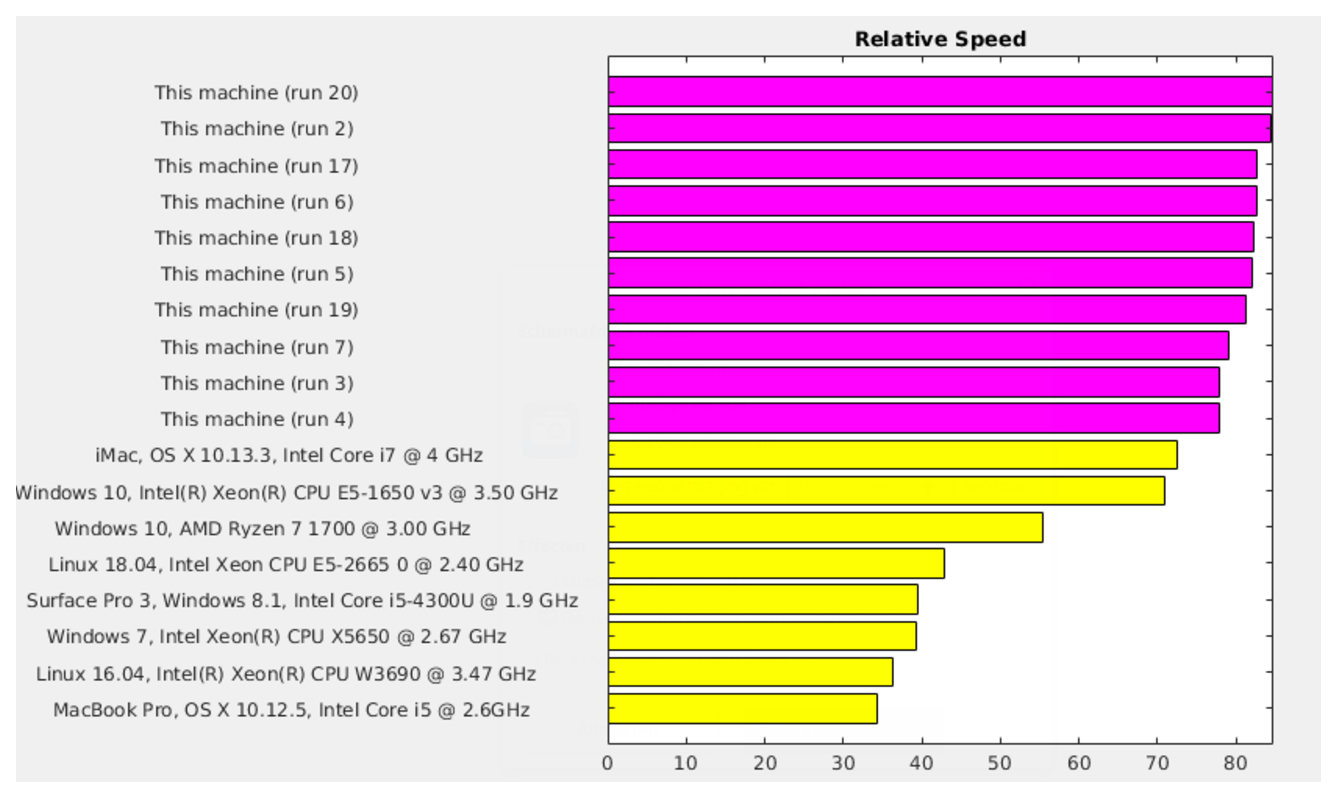
\includegraphics[width=\linewidth]{figures/Performance_1.eps}
    \centering
\end{figure}

\begin{figure}[h!]
    \includegraphics[width=\linewidth]{figures/Performance_2.eps}
    \centering
\end{figure}

\noindent As can bee seen, the performance of the test machine is generally very high. The second thing to note is that the performance varies quite significantly, sometimes as much as about $33 \%$. That is why this benchmark was run $20$ times, even though it only shows the results from the $10$ best runs.
\chapter{Initial implementation}

\lstinputlisting{code/MLDU_Simple.m}

\noindent The block MLDU algorithm was implemented using MATLAB. It represents a typical first attempt without many optimizations. It uses pre-allocation for the output matrices and a nested function for the splitting of the matrix.

\section{Verification and performance analysis}

A simple test was required to verify the correctness of the implementation of the algorithm and analyze its performance. The following code was used:

\lstinputlisting{code/Test_Function_1.m}
\lstinputlisting{code/Matrix_A.m}

\vspace{5mm}

\newpage
\noindent As an example, matrix A and s are provided below ($n = 4$): 

$$
A = 
\left\lbrack\begin{array}{rrrr|rrrr|rrrr|rrrr}
           4&          -1&           0&           0&          -1&           0&           0&           0&           0&           0&           0&           0&           0&           0&           0&           0\\
          -1&           4&          -1&           0&           0&          -1&           0&           0&           0&           0&           0&           0&           0&           0&           0&           0\\
           0&          -1&           4&          -1&           0&           0&          -1&           0&           0&           0&           0&           0&           0&           0&           0&           0\\
           0&           0&          -1&           4&           0&           0&           0&          -1&           0&           0&           0&           0&           0&           0&           0&           0\\ \hline
          -1&           0&           0&           0&           4&          -1&           0&           0&          -1&           0&           0&           0&           0&           0&           0&           0\\
           0&          -1&           0&           0&          -1&           4&          -1&           0&           0&          -1&           0&           0&           0&           0&           0&           0\\
           0&           0&          -1&           0&           0&          -1&           4&          -1&           0&           0&          -1&           0&           0&           0&           0&           0\\
           0&           0&           0&          -1&           0&           0&          -1&           4&           0&           0&           0&          -1&           0&           0&           0&           0\\ \hline
           0&           0&           0&           0&          -1&           0&           0&           0&           4&          -1&           0&           0&          -1&           0&           0&           0\\
           0&           0&           0&           0&           0&          -1&           0&           0&          -1&           4&          -1&           0&           0&          -1&           0&           0\\
           0&           0&           0&           0&           0&           0&          -1&           0&           0&          -1&           4&          -1&           0&           0&          -1&           0\\
           0&           0&           0&           0&           0&           0&           0&          -1&           0&           0&          -1&           4&           0&           0&           0&          -1\\  \hline
           0&           0&           0&           0&           0&           0&           0&           0&          -1&           0&           0&           0&           4&          -1&           0&           0\\
           0&           0&           0&           0&           0&           0&           0&           0&           0&          -1&           0&           0&          -1&           4&          -1&           0\\
           0&           0&           0&           0&           0&           0&           0&           0&           0&           0&          -1&           0&           0&          -1&           4&          -1\\
           0&           0&           0&           0&           0&           0&           0&           0&           0&           0&           0&          -1&           0&           0&          -1&           4\\
\end{array}\right\rbrack
$$

$$
s =
\left\lbrack\begin{array}{rrrrrrrr}
           2&           2&           2&           2&           2&           2&           2&           2\\
\end{array}\right\rbrack
$$

\noindent Running the test with $n = 100$ creates a $10.000 \times 10.000$ matrix. Calculating the Frobenius norm of the error results in:

\vspace{5mm}

\noindent \texttt{>> [ E ] = Test\_Function\_1( 100, @MLDU\_Simple )}\\
\\
\texttt{E =}\\
\\
\texttt{   1.1409e-13}

\vspace{5mm}

\noindent The resulting error is small enough to be confident in the correct operation of the implementation, at least for this test case.

\vspace{5mm}

\noindent Running the profiler with the same input results in the following table:

\begin{figure}[h!]
    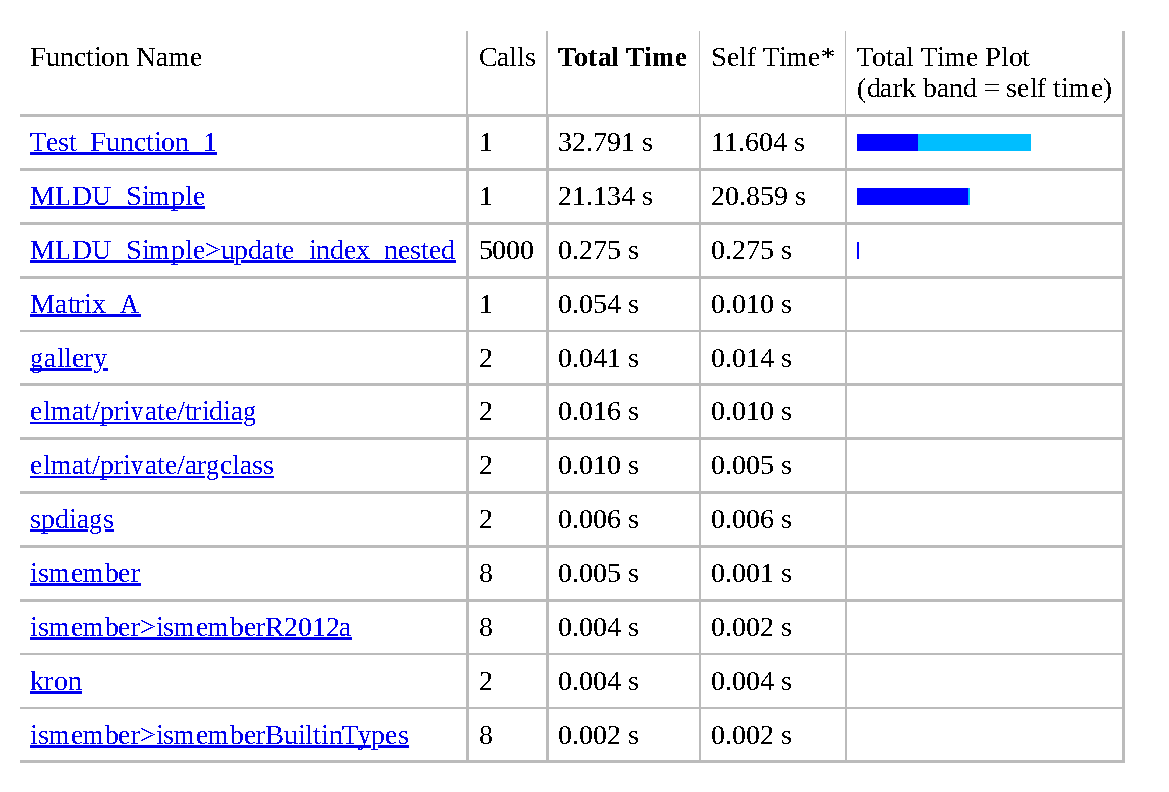
\includegraphics[width=\linewidth]{figures/Profile_MLDU_Simple_1.eps}
    \centering
\end{figure}

\noindent The first thing to note is that the runtime is about $30$ seconds for this test case, of which roughly $20$ seconds are spend by the \texttt{MLDU\_Simple} function. A $10.000 \times 10.000$ matrix is not really small, but it's not large either. As such, $20$ seconds to provide the factorization is a rather poor result.

\newpage

\noindent To get a better understanding of what is going on, the following profiler information was pulled up:

\begin{figure}[h!]
    \includegraphics[width=0.95\linewidth]{figures/Profile_MLDU_Simple_2.eps}
    \centering
\end{figure}

\noindent About 12 seconds of the runtime are spent calculating the Frobenius norm of the error, which can clearly be omitted from the performance analysis. Zooming in on the profiler information of the \texttt{MLDU\_Simple.m} function yields:

\begin{figure}[b!]
    \includegraphics[width=0.95\linewidth]{figures/Profile_MLDU_Simple_3.eps}
    \centering
    \label{Piramid}
\end{figure}

\newpage

\section{Discussion of the results}

\noindent The results mostly speak for themselves. A huge part of the runtime of the implementation is spent on line $27$, where the results of the Schur complement update gets subtracted from the matrix. Even though there are some calculations involved in this line, they could not account for this excessive runtime.\\

\noindent Calculating the Schur complement happens at lines $23$, $24$ and $25$, which takes about $1.5$ seconds. Most of that time is not actually spent doing any calculations, but rather accessing the elements of matrix \texttt{U}. This is to be expected, as the sparse storage format of MATLAB is catered towards accessing columns rather than rows. Further proof of this can be found at line $21$, where separating the elements of \texttt{U} from \texttt{A} actually takes more time than calculating the Schur complement update.\\

\noindent The point is that most of the runtime of line $27$ will most likely be spent on the memory operations associated with inserting columns and rows of data into an existing sparse matrix. There are a couple of obvious possibilities that might be tried to circumvent this problem:

\begin{itemize}
    \item Switch from sparse to full matrix storage.
    \item Store rows in a transposed fashion.
    \item Use a matrix storage format that doesn't require as many memory operations to insert rows and columns.
\end{itemize}

\noindent The first possibility may seem silly, but is not as stupid as may at first appear. Fill-in is a real nemesis of algorithms like Block MLDU, and can make a sparse matrix very full in some instances. Switching to full matrix storage in these situations makes perfect sense and will provide a very healthy performance improvement.\\

\noindent Storing the rows as transposed columns can have tangible benefits, but it has certain disadvantages as well. The most obvious downside is the extra memory consumption, as the matrix will probably need to be stored twice. The second problem is that the block nature of the algorithm makes a lot of the work required to adapt the code that much harder.\\
\noindent It should be noted that this possible improvement should definitely be investigated further, as it could be a huge advantage in situations where the input matrix is symmetric.\\

\noindent Switching to a different matrix storage format will probably provide the most benefits, especially if the storage format is designed from scratch and tailored to the needs of the Block MLDU algorithm. The second implementation of the algorithm will focus on this possibility.

\chapter{Reduced memory consumption}

The initial implementation has a couple of problems, one of which is it's memory consumption. This excessive memory consumption is mostly caused by the implementation of the memory preallocation for the matrices \texttt{L}, \texttt{D} and \texttt{U}. Using \texttt{zeros(m,n)} results in full matrices for \texttt{L}, \texttt{D} and \texttt{U}, while they are often far from full.\\

\noindent The painful part is the fact that matrices \texttt{L}, \texttt{D} and \texttt{U} grow dynamically with each iteration of the \texttt{for}-loop. Adding to the problem is that fill-in makes it impossible to know a priory by just how much they grow each iteration. Memory preallocation is a real pig in these type of situations and resorting to a full \texttt{zeros} matrix is often the only way that doesn't involve very complicated or convoluted code.\\

\noindent Dynamic growth of a matrix in a \texttt{for}-loop is evil, mostly because matrices require a contiguous memory block. Adding data to a matrix involves allocating an entirely new contiguous block of memory for the matrix, copying the old values from the previous block to the new, then releasing the old block for potential reuse. These memory operations are time consuming and should be avoided in \texttt{for}-loops. The most common way to deal with this problem is to use memory preallocation, but the other possibility is to use a data structure that drops the contiguous memory range requirement.\\

\noindent With an eye on making the implementation more memory efficient for a variety or reasons, an effort was undertaken to tackle the problem. As stated earlier, preallocation is difficult to achieve. With this in mind, the plan was to NOT use memory preallocation, but instead write the code in such a way that the negative effects of not using memory preallocation are largely avoided. MATLAB has a data structure known as a "cell array"\autocite[]{math_doc_cell}, the most obvious differentiating qualities between it and a matrix data structure are:

\begin{itemize}
    \item Can contain different kind of elements. A collection of an "int", a matrix and a string can all be stored in the same cell array.
    \item No contiguous memory range required. The separate entries of the cell array may require a contiguous memory range, but the collection of the entries might be stored separately.
\end{itemize}

\noindent The most obvious quality that cell arrays and matrices share is their ability to be indexed, something that a "struct" lacks\autocite[]{math_doc_struct}. The improved implementation uses cell arrays to store the additions of the matrices \texttt{L}, \texttt{D} and \texttt{U}, with each element of the cell array containing a COO representation of the \texttt{for}-loop additions\autocite[]{wiki_coo}.\\

\section{The code}

\lstinputlisting{code/MLDU_Simple_cell.m}

\section{Discussion of the code}

This implementation creates one new nested function, two new local functions and increases the number of lines from $47$ to $91$, so the reduced memory consumption does come at the cost of code complexity.

\newpage

\section{Profiler results}

\noindent The profiler results below are generated by running:\\

\noindent \texttt{[ E ] = Test\_Function\_1( 100, @MLDU\_Simple\_cell )}\\

\begin{figure}[h!]
    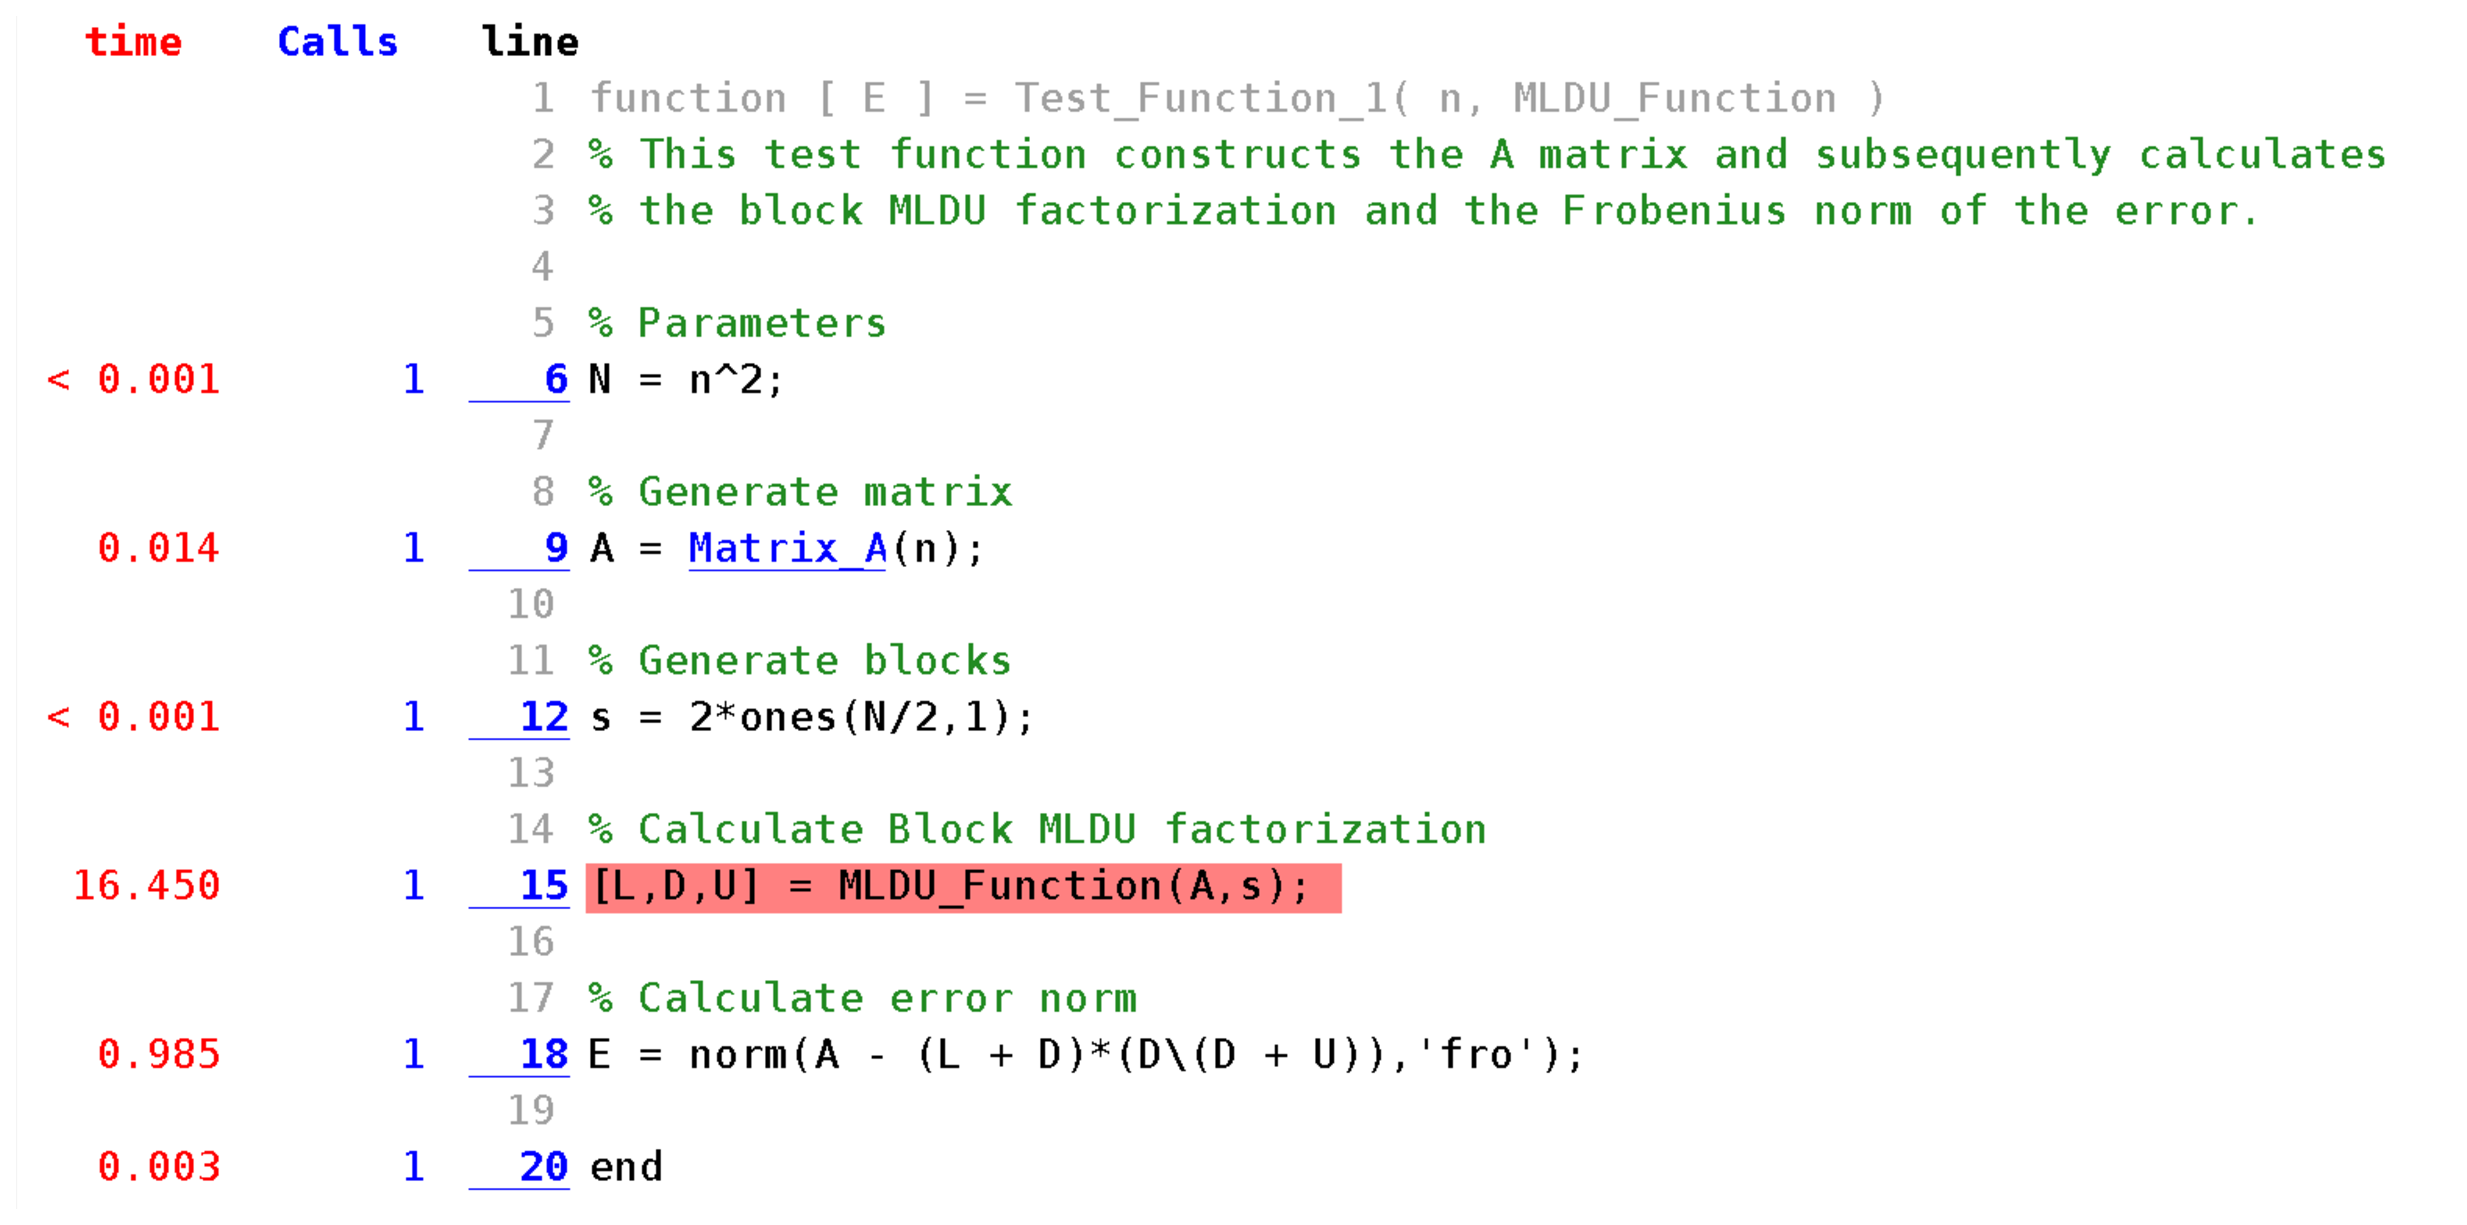
\includegraphics[width=\linewidth]{figures/Profile_MLDU_Simple_cell_1.eps}
    \centering
\end{figure}

\noindent This is exactly the same as the previous situation. The error is also acceptable:\\

\noindent \texttt{E =}\\
\\
\noindent \texttt{   1.1287e-13}\\

\noindent Apart from the targeted result that the memory consumption has decreased, a couple of other noteworthy positive changes occurred as well.\\

\noindent One of the positive aspect is that calculating the error has a vastly reduced runtime, from about $10$ seconds to just under one second. This is caused by the fact that matrices \texttt{L}, \texttt{D} and \texttt{U} are now sparse, making the calculation a lot faster.

\begin{figure}[h!]
    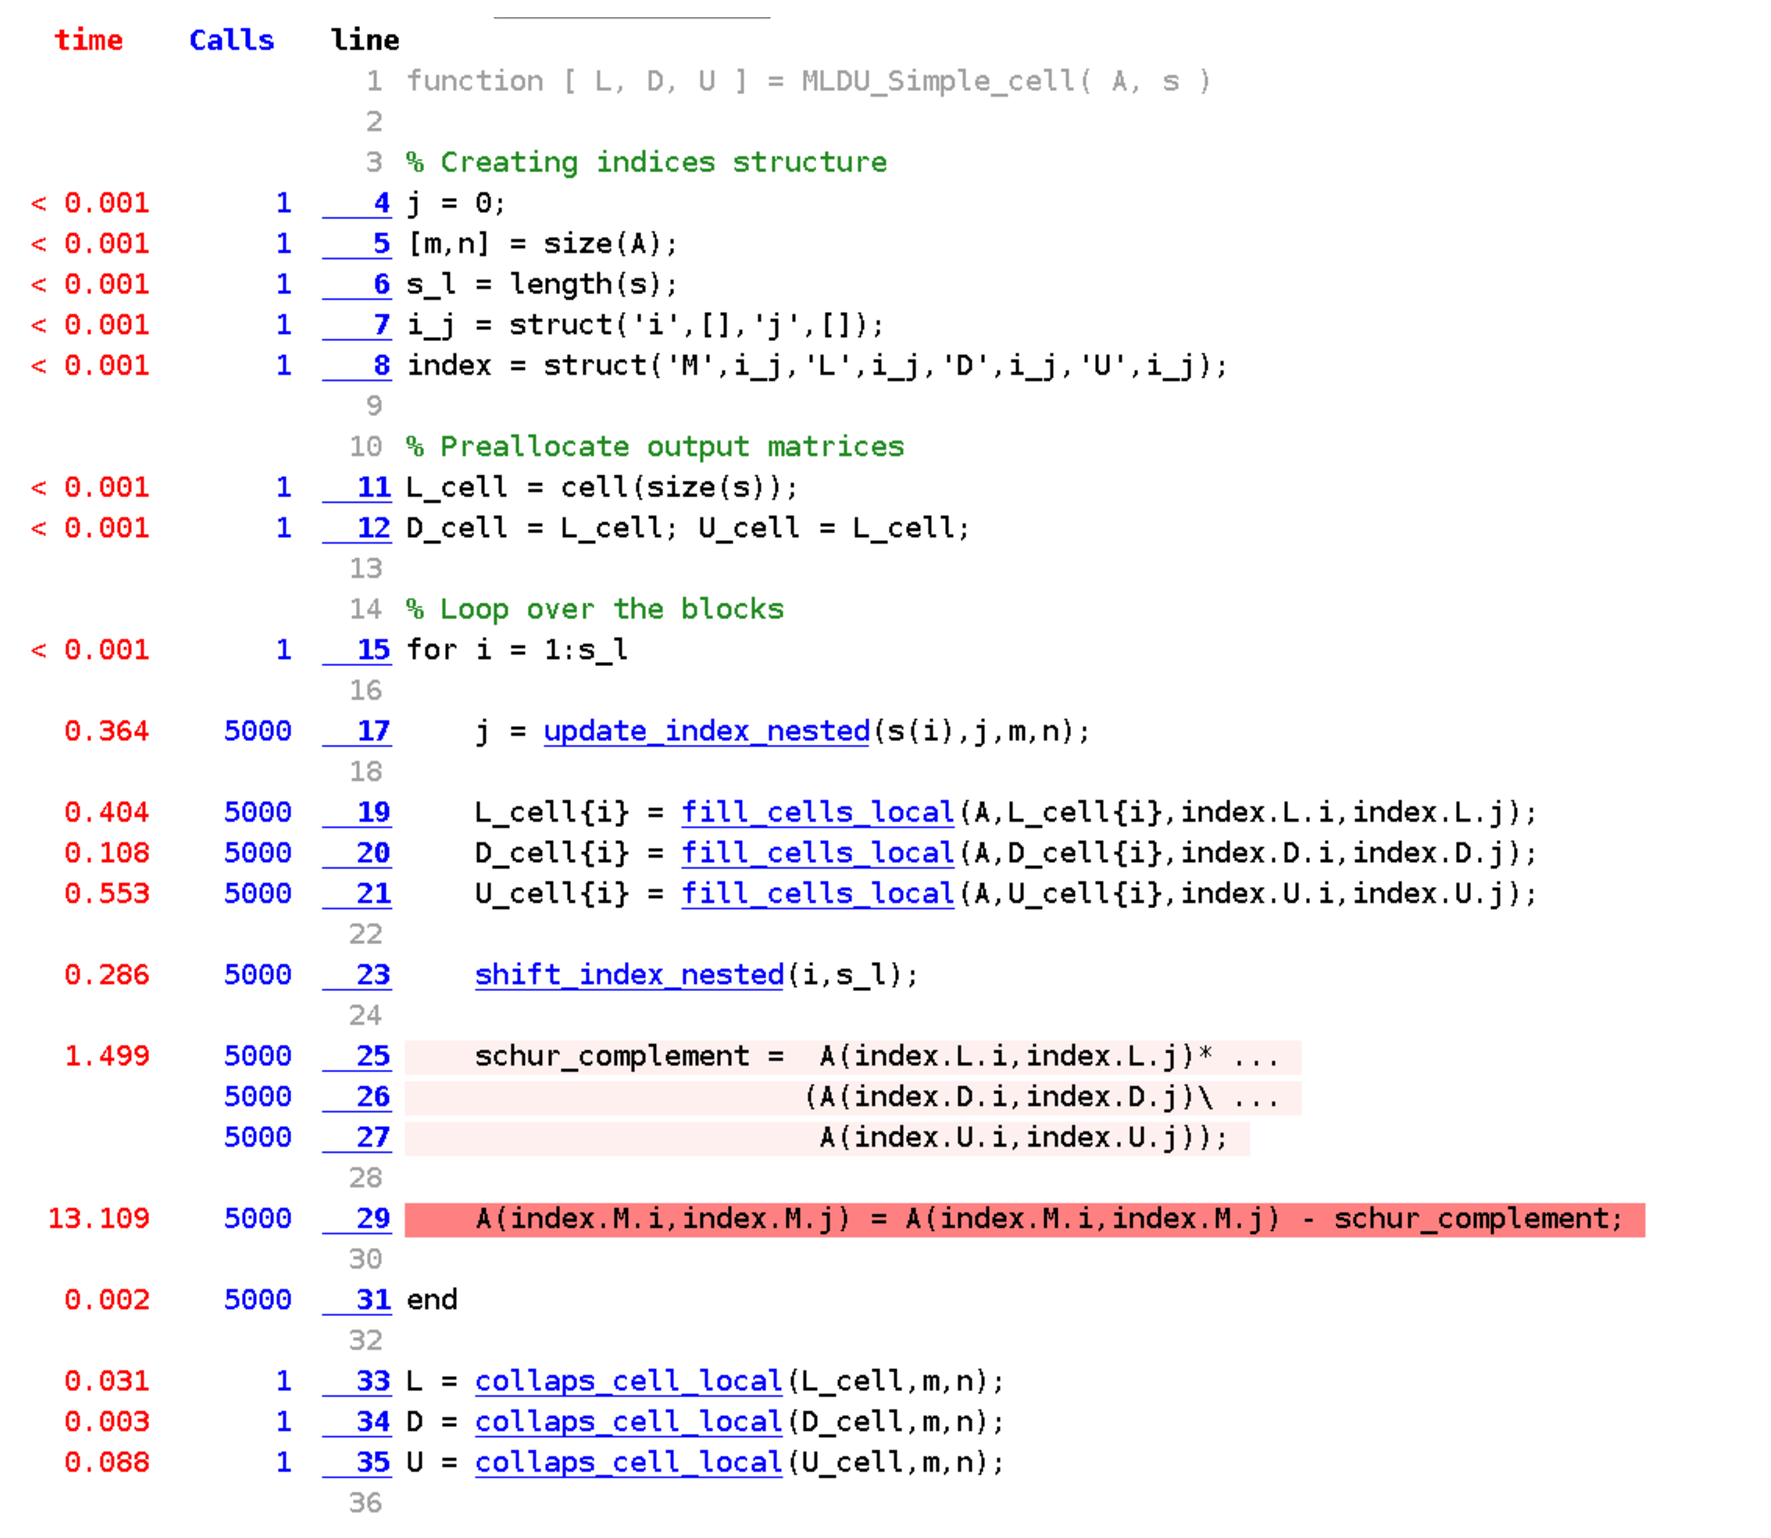
\includegraphics[width=\linewidth]{figures/Profile_MLDU_Simple_cell_2.eps}
    \centering
\end{figure}

\noindent The runtime required to save the matrices \texttt{L}, \texttt{D} and \texttt{U} has actually decreased. The initial implementation spends $2.243$ seconds at lines $19$ through $21$ while the cell array implementation takes a total of $1.187$ seconds at lines $19, 20, 21$ and $33, 34, 35$.\\

\noindent Lastly and maybe the most significant side effect of the cell array implementation is the runtime reduction of line $26$, from about $17$ seconds to about $13$ seconds, a reduction of about $25 \%$. This is probably caused by the reduced memory consumption itself, allowing the cache of the CPU to operate more effectively.
\chapter{Increased memory bandwidth}

Line $29$ of the function \texttt{MLDU\_Simple\_cell} is the obvious bottleneck of the implementation. This line gets called every iteration of the \texttt{for} loop and adds data to the matrix \texttt{A}. This addition of data requires many memory operations, which makes it slow. The performance of the main memory subsystem of a computer is comprised of two aspects, bandwidth and latency. Bandwidth is a measure of maximum throughput and latency is a measure of the access time.\\

\noindent This chapter tries to shed some light on which of the two main memory performance indicators is to blame for the poor performance of line $29$.

\section{GPU}

The GPU is interesting in this scenario because dedicated GPU's contains VRAM. Comparing VRAM to standard RAM, which makes up the main memory of a computer, reveals that VRAM has a much higher bandwidth than RAM. The downside is that VRAM has a somewhat higher latency than RAM.\\

\noindent Implementing the block MLDU algorithm on the GPU would make it possible to identify whether latency or bandwidth is to blame for the poor runtime of line $29$. A bandwidth bottleneck would result in a faster execution of line $29$ and a latency bottleneck would cause it to be slightly slower then on the CPU.

\section{MATLAB Sparse gpuArray limitations}

MATLAB facilitates GPGPU programming, but has limitations, especially when it comes to sparse matrices. The most notable limitations for the block MLDU algorithm are the inability to index in sparse gpuArrays and the fact that the "\textbackslash" operator is not feature complete.\\

\noindent These limitations make it very unappealing to write a "simple" MATLAB implementation of the block MLDU algorithm on the GPU. The overall performance will almost certainly be slower than the CPU implementation, because all the hacks required to get it functional will swamp any floating point performance benefits that the GPU has over the CPU.\\

\noindent Regardless, it will provide insight into the latency versus bandwidth question and as such is still valuable to this project.

\newpage

\subsection{The code}

\lstinputlisting{code/MLDU_Simple_GPU.m}

\subsection{Profiler results}

\noindent The profiler results below are generated by running:\\

\noindent \texttt{[ E ] = Test\_Function\_1( 40, @MLDU\_Simple\_GPU )}\\

\noindent The total runtime of this reduced size test was about $16$ seconds, which is way slower than the \texttt{MLDU\_Simple\_cell} implementation, which takes about $0.4$ seconds. The error of \texttt{MLDU\_Simple\_GPU} was again reasonable at $2.9072e-14$.

\begin{figure}[h!]
    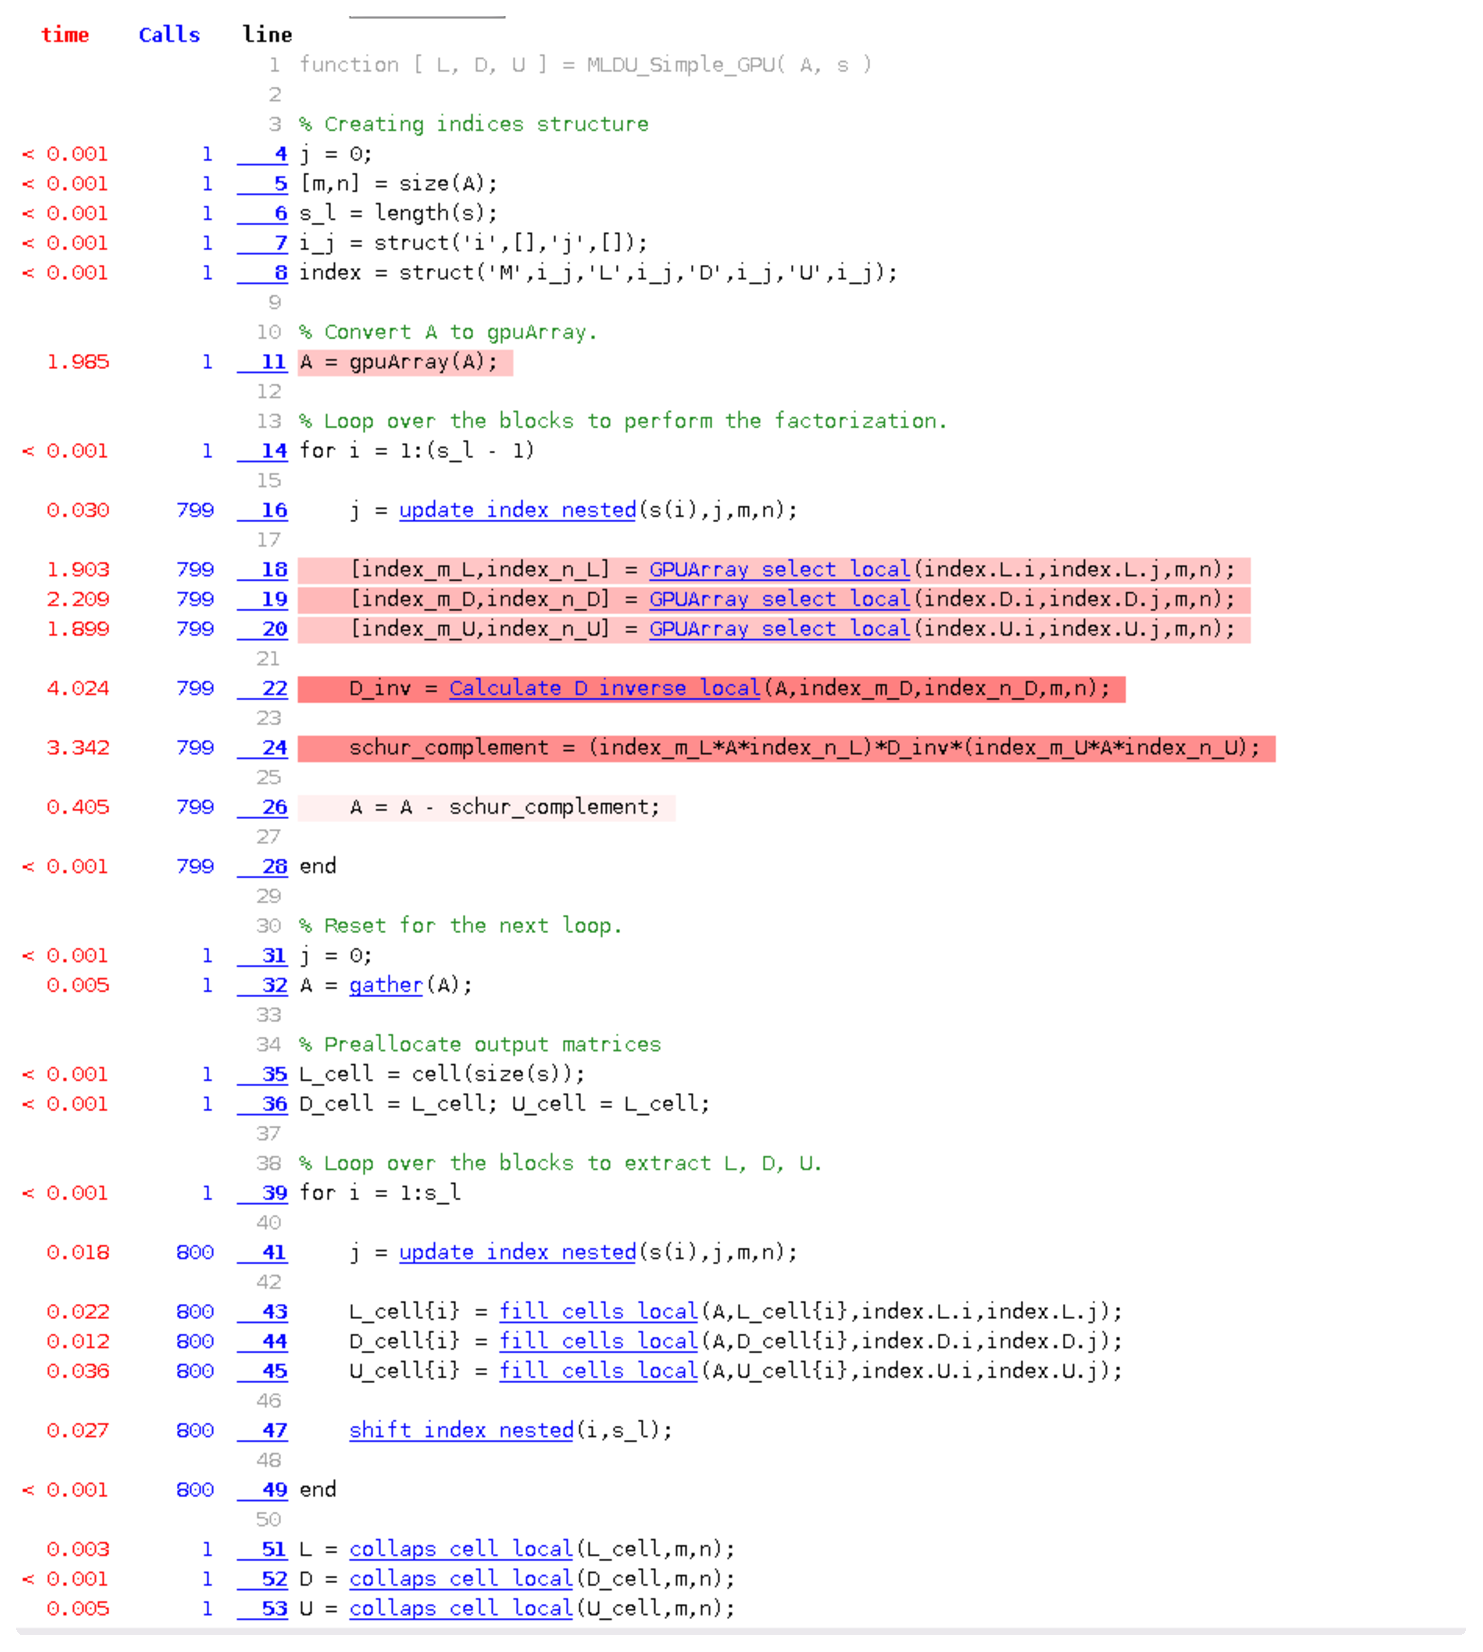
\includegraphics[width=\linewidth]{figures/Profile_MLDU_Simple_GPU_1.eps}
    \centering
\end{figure}

\newpage

\noindent The most interesting timing result for this discussion is that of line $26$ (above), which has a value of $0.405$. Line $29$ of \texttt{MLDU\_Simple\_cell} executes the same operation, but takes only $0.164$ seconds.\\

\noindent The profiler results of \texttt{[ E ] = Test\_Function\_1( 40, @MLDU\_Simple\_cell )} are provided below:

\begin{figure}[h!]
    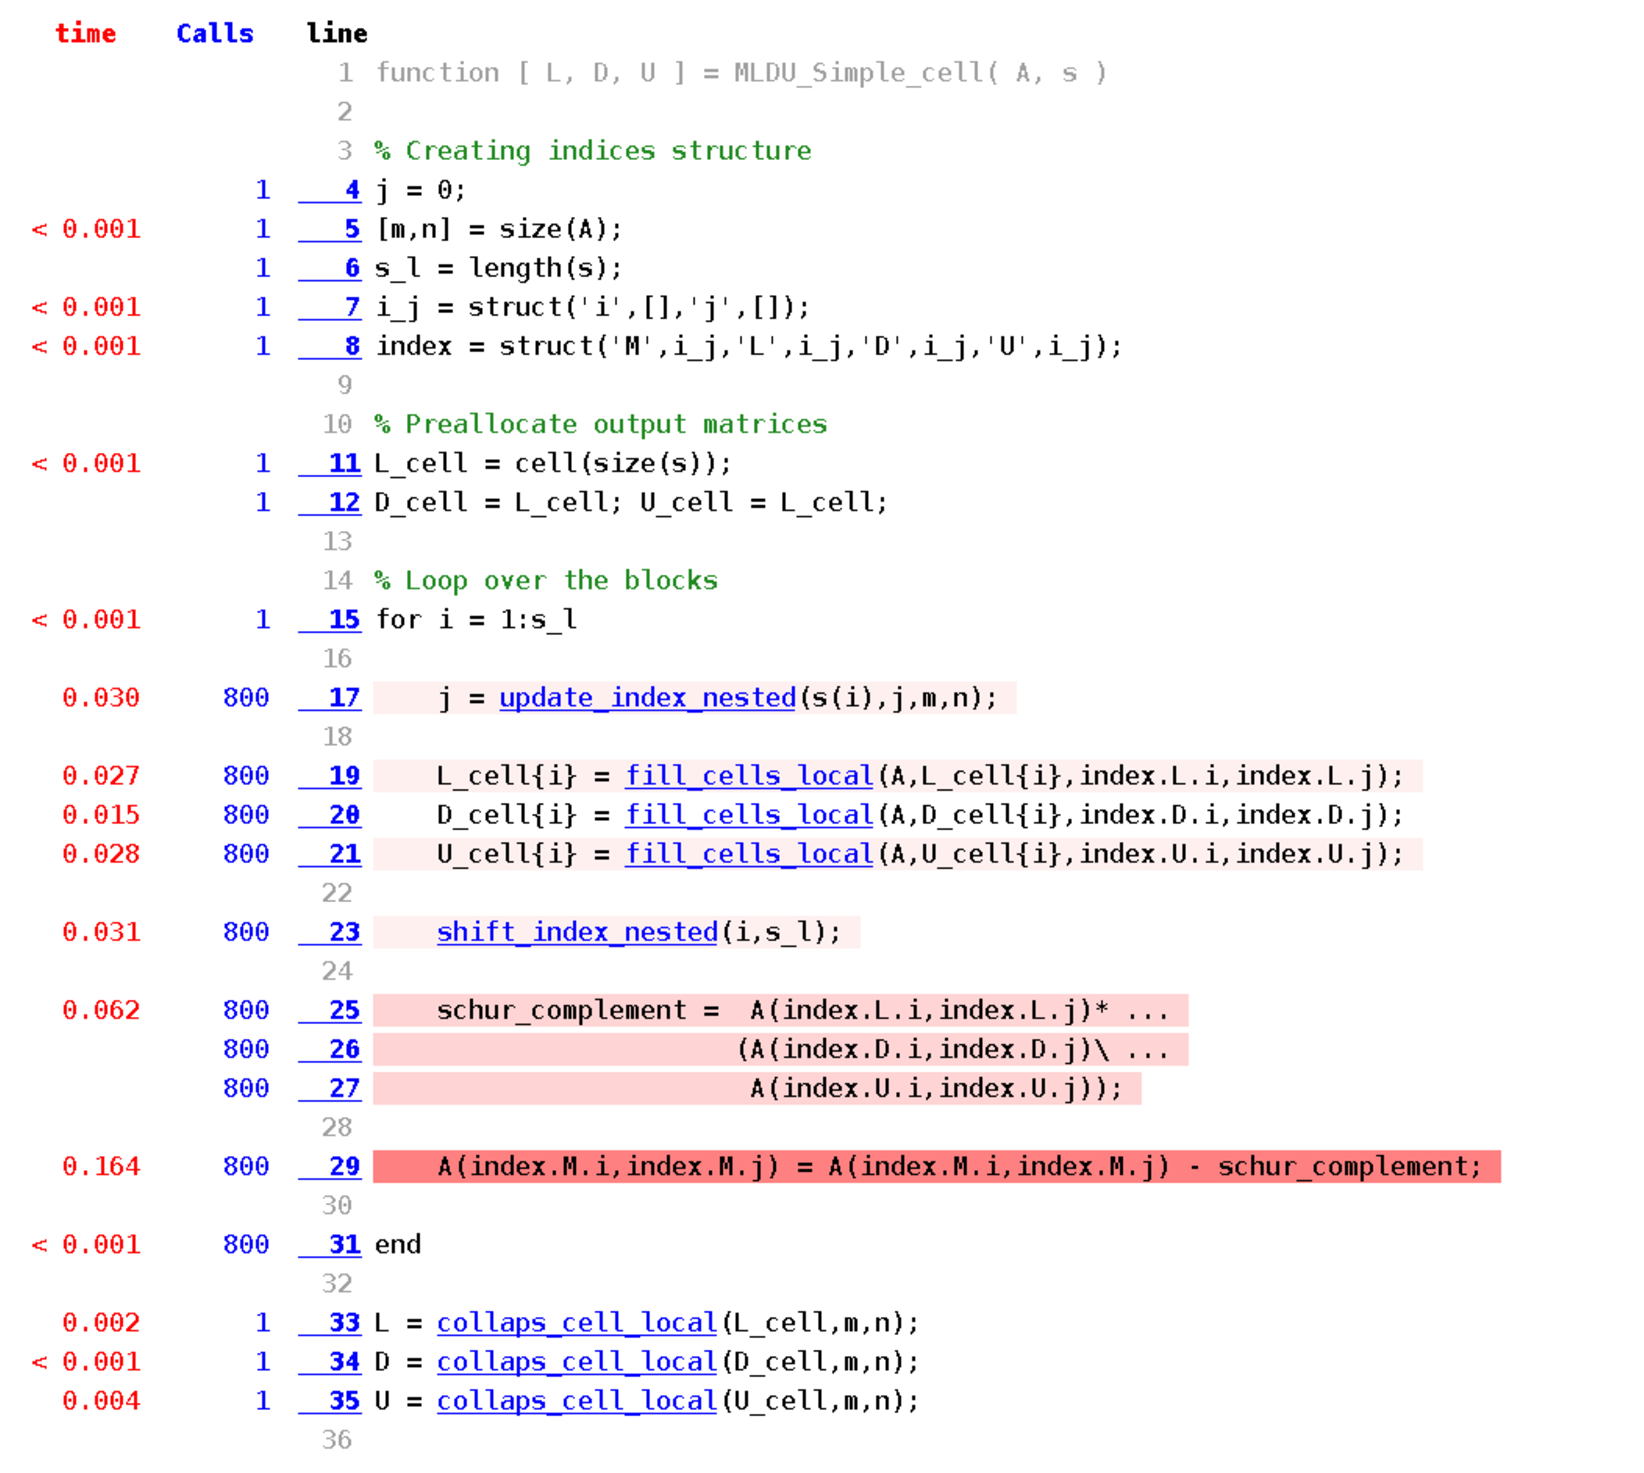
\includegraphics[width=\linewidth]{figures/Profile_MLDU_Simple_GPU_2.eps}
    \centering
\end{figure}

\noindent The clear result from \texttt{MLDU\_Simple\_GPU} is that it does not constitute an improvement. This may very well be down to the limiting aspects of MATLAB sparse gpuArrays, but further investigation would be required to know for certain. The second lesson from \texttt{MLDU\_Simple\_GPU} is that the operation at line $29$ or $26$ is latency bound.
\chapter{Conclusion}

The goal of this Capita Selecta is to investigate the possibilities for a fast MATLAB based implementation of the Block MLDU algorithm. The most distinguishing drawback of using MATLAB for high performance code is its interpreter overhead.\\

\noindent The implementations provided in this report are not particularly fast, but they do indicate one thing. Because almost all of the runtime of the implementation is spent on a single MATLAB statement, it can be concluded that the interpreter overhead of MATLAB is not to blame for the disappointing runtime.\\

\noindent Finding that the MATLAB interpreter is not the performance bottleneck, incentivized further research into a MATLAB implementation of the Block MLDU algorithm. This research has shown that the bottleneck is the storing operation of the Schur complement update into the matrix. Fill-in is the ultimate culprit of this problem, because it requires freeing extra memory for the additional non-zero elements. The memory operations required are DRAM latency bound and as such are very hard to accelerate.\\

\noindent It should be noted that an incomplete version of the Block MLDU algorithm would not suffer the aforementioned problems, and as such could easily be implemented in a high performance manner using a similar approach as provided in this report.\\

\noindent The conclusion of this Capita Selecta is that the default sparse matrix storage format (CCS) of MATLAB is sub optimal for this algorithm. Large performance gains should be possible if a matrix storage format was selected that circumvents the costly memory freeing operations associated with the Schur complement update.\\

\noindent One possible alternative to CCS would be COO, as it is more flexible. It's main advantage in this situation is the fact that the order in which the matrix entries are stored, does not alter the location of the entries in the matrix. This should circumvent the need for all the memory freeing operations that are currently frustration the performance.\\

\noindent The main challenge of the COO approach is searching through the elements of the matrix during the matrix splitting step of the algorithm. The lack of ordering in the COO format causes these operations to be much slower than in the CCS situation, so finding a way around this problem will again provide great performance improvements. 

% Bibliography
\cleardoublepage
\printbibliography

\end{document}